\def\pgfsysdriver{pgfsys-dvisvgm.def}
% flashcards-title: Three roles of biological information
% flashcards-desc: Panel A shows a pattern held over time, Panel B a change moving between components, and Panel C a cue changing a detector.
\documentclass[tikz,border=6pt]{standalone}
\usetikzlibrary{arrows.meta,calc,fit,positioning,shapes.geometric}

\definecolor{fcink}{HTML}{17212B}
\definecolor{fcblue}{HTML}{1D5D8C}
\definecolor{fcgreen}{HTML}{2D6A4F}
\definecolor{fcorange}{HTML}{A44A1F}
\definecolor{fcpale}{HTML}{F4F7F9}
\definecolor{fcsoil}{HTML}{8B5E3C}

\tikzset{
  fc text/.style={font=\sffamily, text=fcink},
  fc panel/.style={draw=fcink, line width=0.9pt, rounded corners=5pt, fill=fcpale},
  fc node/.style={draw=fcink, line width=0.9pt, rounded corners=4pt, fill=white,
    minimum width=24mm, minimum height=10mm, align=center, font=\sffamily},
  fc arrow/.style={-{Stealth[length=3.2mm,width=2.4mm]}, line width=1.2pt,
    draw=fcblue, line cap=butt},
  fc boundary/.style={draw=fcorange, line width=1.4pt, dash pattern=on 5pt off 3pt,
    rounded corners=7pt},
  fc label/.style={font=\sffamily\bfseries, text=fcink},
  fc note/.style={font=\sffamily\small, text=fcink, align=center}
}

\begin{document}
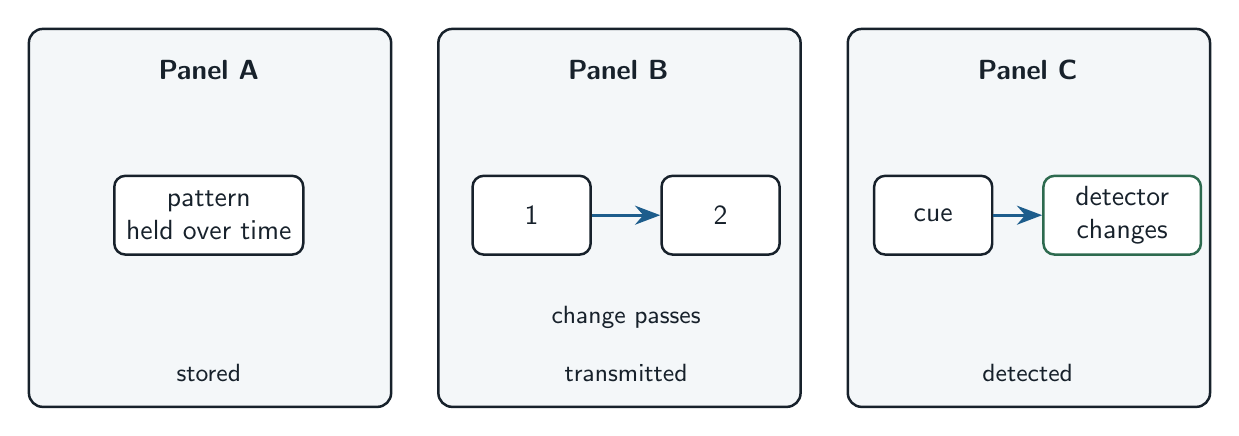
\begin{tikzpicture}[fc text, x=1cm, y=1cm]
  \foreach \x/\lab in {0/A,5.2/B,10.4/C} {
    \node[fc panel, minimum width=46mm, minimum height=48mm, anchor=south west] at (\x,0) {};
    \node[fc label] at (\x+2.3,4.3) {Panel \lab};
  }
  \node[fc node] at (2.3,2.45) {pattern\\held over time};
  \node[fc node, minimum width=15mm] (b1) at (6.4,2.45) {1};
  \node[fc node, minimum width=15mm] (b2) at (8.8,2.45) {2};
  \draw[fc arrow] (b1)--(b2);
  \node[fc note] at (7.6,1.15) {change passes};
  \node[fc node, minimum width=15mm] (c1) at (11.5,2.45) {cue};
  \node[fc node, minimum width=20mm, draw=fcgreen] (c2) at (13.9,2.45) {detector\\changes};
  \draw[fc arrow] (c1)--(c2);
  \node[fc note] at (2.3,0.45) {stored};
  \node[fc note] at (7.6,0.45) {transmitted};
  \node[fc note] at (12.7,0.45) {detected};
\end{tikzpicture}
\end{document}
